%Техмейкер: пдфлатех→мейкиндекс→пдфлатех→пдфлатех
\documentclass[a4paper,12pt]{article}

%%% Работа с русским языком
%\usepackage{DejaVuSans}
\usepackage{cmbright}
%\usepackage[OT1]{fontenc}
\renewcommand*\familydefault{\sfdefault} %% Only if the base font of the document is to be sans serif
\usepackage{cmap}					% поиск в PDF
\usepackage{mathtext} 				% русские буквы в формулах
\usepackage[T2A]{fontenc}			% кодировка
\usepackage[utf8]{inputenc}			% кодировка исходного текста
\usepackage[english]{babel}	% локализация и переносы
\usepackage{indentfirst}            % красная строка в первом абзаце
\usepackage{mathtext} 				% русские буквы в формулах
\frenchspacing                      % равные пробелы между словами и предложениями



%Добавлено:
\usepackage{refcount} 				% перекрёстные ссылки внутри документа
\usepackage{fixfoot,xspace}			% двойная ссылка
\usepackage{tipa}					% греческие в тексте
\usepackage{dcolumn}				% выравнивание по точке
\usepackage{mhchem} 				% Оформление химических формул
%\usepackage{acro}					% ведение списка сокращений
%\AddAcroTranslations{Russian}{list-name = Список сокращений} 	% Что будет написано в заголовке
\usepackage{caption}				% несколько рисунков
\usepackage{subcaption}				% несколько рисунков
\usepackage{gensymb}				% градусы цельсия
\usepackage{multicol}				% Текст в две колонки
\usepackage{siunitx}				% работа с цифрами
\usepackage{wrapfig}				% обтекание рисунков текстом
\usepackage[inline]{enumitem}		%Горизонтальный список, добавлется звёздочкой

%Добавленные команды
\newcommand{\grad}{~\celsius}

% \makeatletter									%Подпись к рисункам Рисунок, вместо Рис
% \renewcommand{\fnum@figure}{Рисунок \thefigure}
% \makeatother
% %\counterwithin{figure}{section}

\renewcommand{\labelenumii}{\arabic{enumi}.\arabic{enumii}}	% отвечает за уровень списка
\renewcommand{\labelenumiii}{\arabic{enumi}.\arabic{enumii}.\arabic{enumiii}}
\renewcommand{\labelenumiv}{\arabic{enumi}.\arabic{enumii}.\arabic{enumiii}.\arabic{enumiv}}

% \addto\captionsrussian{% Replace "english" with the language you use
%   \renewcommand{\contentsname}{Table of Contents}}%%Подпись к оглавлению



%%% Шаблонная информация для титульного листа
\newcommand{\CourseName}{}
\newcommand{\FullCourseNameFirstPart}{\so{}}
\newcommand{\SemesterNumber}{}
\newcommand{\LecturerInitials}{}
\newcommand{\CourseDate}{2023}

%%% Оформление страницы
\usepackage{extsizes}     % Возможность сделать 14-й шрифт
\usepackage{geometry}     % Простой способ задавать поля
\usepackage{setspace}     % Интерлиньяж
\usepackage{enumitem}     % Настройка окружений itemize и enumerate
\setlist{leftmargin=25pt} % Отступы в itemize и enumerate

\geometry{top=15mm}    % Поля сверху страницы
\geometry{bottom=30mm} % Поля снизу страницы
\geometry{left=15mm}   % Поля слева страницы
\geometry{right=15mm}  % Поля справа страницы

\setlength\parindent{15pt}        % Устанавливает длину красной строки
\linespread{1.1}                  % Коэффициент межстрочного интервала
%\setlength{\parskip}{0.2em}      % Вертикальный интервал между абзацами
%\setcounter{secnumdepth}{0}      % Отключение нумерации разделов
%\setcounter{section}{-1}         % Нумерация секций с нуля
\usepackage{multicol}			  % Для текста в нескольких колонках
\usepackage{soulutf8}             % Модификаторы начертания

%%% Добавлено:
\usepackage{parskip} % сам настроит интервалы нужным образом
\setlength{\parindent}{0,8cm} % по умолчанию — 0

%%% Колонтитулы
\usepackage{titleps}
\newpagestyle{main}{
	\setheadrule{0pt}
%	\sethead{\subsectiontitle}{}{\hyperlink{intro}{\;К содержанию}}
	\setfootrule{0pt}                       
	\setfoot{}{}{\thepage} 
}
\pagestyle{main} 

%%% Дополнительная работа с математикой
\usepackage{amsmath,amsfonts,amssymb,amsthm,mathtools} % пакеты AMS
\usepackage{icomma}                                    % "Умная" запятая

%\newcommand{\dse}{\displaystyle}

%%% Перенос знаков в формулах (по Львовскому)
%\newcommand*{\hm}[1]{#1\nobreak\discretionary{}{\hbox{$\mathsurround=0pt #1$}}{}}

%%% Работа с картинками
\usepackage{graphicx}    % Для вставки рисунков
\setlength\fboxsep{3pt}  % Отступ рамки \fbox{} от рисунка
\setlength\fboxrule{1pt} % Толщина линий рамки \fbox{}
\usepackage{wrapfig}     % Обтекание рисунков текстом

%%% Работа с таблицами
\usepackage{array,tabularx,tabulary,booktabs} % Дополнительная работа с таблицами
\usepackage{longtable}                        % Длинные таблицы
\usepackage{multirow}                         % Слияние строк в таблице
\usepackage{makecell}						% Перенос в ячейках строк
%\usepackage{tablefootnote}					% Сноски в таблицах (работает плохо)
\usepackage{booktabs,caption}				% Сноски под таблицей
\usepackage[flushleft]{threeparttable}		% Сноски под таблицей


%%% Теоремы
\theoremstyle{plain}
\newtheorem{theorem}{Теорема}[section]
\newtheorem{lemma}{Лемма}[section]
\newtheorem{proposition}{Утверждение}[section]
\newtheorem*{exercise}{Упражнение}

\theoremstyle{definition}
\newtheorem{definition}{Определение}[section]
\newtheorem*{adefinition}{Определение(не материал лектора)}
\newtheorem*{corollary}{Следствие}
\newtheorem*{addition}{Дополнение}
\newtheorem*{note}{Замечание}
\newtheorem*{anote}{Замечание автора}
\newtheorem*{reminder}{Напоминание}
\newtheorem{example}{Пример}
\newtheorem*{examples}{Примеры}

\theoremstyle{remark}
\newtheorem*{solution}{Решение}


 

% %%% Нумерация уравнений
% \makeatletter
% \def\eqref{\@ifstar\@eqref\@@eqref}
% \def\@eqref#1{\textup{\tagform@{\ref*{#1}}}}
% \def\@@eqref#1{\textup{\tagform@{\ref{#1}}}}
% \makeatother                      % \eqref* без гиперссылки
% \numberwithin{equation}  % Нумерация вида (номер_секции).(номер_уравнения)
% \mathtoolsset{showonlyrefs=false} % Номера только у формул с \eqref{} в тексте.

%%% Гиперссылки
\usepackage{hyperref}
\usepackage[usenames,dvipsnames,svgnames,table,rgb]{xcolor}
\hypersetup{
	unicode=true,            % русские буквы в раздела PDF
	colorlinks=true,       	 % Цветные ссылки вместо ссылок в рамках
	linkcolor=black!15!blue, % Внутренние ссылки
	citecolor=green,         % Ссылки на библиографию
	filecolor=magenta,       % Ссылки на файлы
	urlcolor=NavyBlue,       % Ссылки на URL
}

%%% Графика
\usepackage{tikz}        % Графический пакет tikz
\usepackage{tikz-cd}     % Коммутативные диаграммы
\usepackage{tkz-euclide} % Геометрия
\usepackage{stackengine} % Многострочные тексты в картинках
\usetikzlibrary{angles, babel, quotes, automata,arrows,calc,positioning}

%%% Xlam
%\usepackage{longtable}
%\newcolumntype{d}[1]{D{.}{.}{#1}}
%\usepackage{paratype}
%\renewcommand{\thefootnote}{\alph{footnote}} % Делает сноски буквами



\usepackage{siunitx} % SI unints and numbers
\usepackage{tabulary} 
\usepackage{pdflscape} % page orientation
\usepackage{array} % wrapping
\usepackage{soul} % for HL
\usepackage{hyperref}

\usepackage{blindtext}
\usepackage{multirow}
\renewcommand{\baselinestretch}{1.0}

\begin{document}
%  \begin{titlepage}
	\clearpage\thispagestyle{empty}
	\centering
	
	\textbf{Саратовский университет \\ Институт химии}
	\vspace{33ex}
	
	{\Large {\textbf{Полимеры в биологически активных системах}}}	% Название предмета
	\vspace{6ex}	
	
	\SemesterNumber\ СЕМЕСТР  
	\vspace{6ex}
	
	Лектор: \textit{\LecturerInitials}
	

	\vfill
	\CourseDate
	\pagebreak
\end{titlepage}
  
  \newpage
  \hypertarget{intro}{}
\begin{scriptsize}
   \setlength\columnsep{50pt}
   \begin{multicols}{2}
%   \tableofcontents
   \end{multicols}
\end{scriptsize}

\makeatletter
\renewcommand{\thefigure}{\textbf{S\@arabic\c@figure}}
\makeatletter
\renewcommand{\thesubsection}{S\@arabic\c@subsection}
\makeatletter
\renewcommand{\thetable}{\textbf{S\@arabic\c@table}}
\makeatletter
\renewcommand{\theequation}{S\@arabic\c@equation}
\makeatletter

\newpage
\thispagestyle{empty}

\begin{Huge} 
\begin{spacing}{0.8}
\noindent \textbf{Imprinted Proteins as a Receptor \\ in Fluorescent Sensing Microplate Assay \\ for Herbicides Determination } 

\noindent Supplementary material \\
\end{spacing}
\end{Huge}
% попробовать HUGE или Huge

\noindent Kirill Yu.\,Presnyakov$^{1}$, 
Ivan S.\,Matlakhov$^{1}$, 
Ivan A.\,Reshetnik$^{1}$, 
Polina M.\,Ilicheva$^{1}$, 
Daria V.\,Tsyupka$^{1}$, 
Daria G.\,Koganova$^{1}$, 
Svetlana A. Mescheryakova$^{1}$,
Tatyana Yu.\,Rusanova$^{1}$, 
Mikhail V.\,Pozharov$^{1}$, 
Daniil D.\,Drozd$^{1}$, 
Pavel S.\,Pidenko$^{1}$, 
Irina Yu.\,Goryacheva$^{1}$,
Natalia A.\,Burmistrova$^{1}$*  

\noindent \textit{$^{1}$ Institute of Chemistry, Saratov State University, Astrakhanskaya Street 83, Saratov, 410012, Russia.} 

\noindent * --- corresponding author, e-mail address: \href{naburmistrova@mail.ru}{naburmistrova@mail.ru}

%Contributing authors: \href{daniild.drozd@yandex.ru}{daniild.drozd@yandex.ru}
%\href{pidenkops@gmail.com}{pidenkops@gmail.com}

\listoftables
\listoffigures

\newpage

\makeatletter
\pagenumbering{roman}


\begin{table}[h] %\centering
\footnotesize
\caption{Maximum permissible levels of imazamox in~cereal plants in different countries}\label{esmTab:MPL}
\begin{tabular}{@{}llll@{}}
\toprule
Country  & Culture  & Concentration limit & Ref.\\
\midrule
Russia     & Sunflower seeds  & 0.004~\unit{\mg\per\cubic\metre}   & \footnotemark[38]  \\
USA        & Wheat            & 0.3 ppm                            & \footnotemark[39]  \\
China      & Wheat            & 0.05~\unit{\mg\per\kilogram}       & \footnotemark[40] \\
Australia  & Barley           & 0.02--0.04~\unit{\mg\per\kilogram} & \footnotemark[41] \\
EU         & Sunflower seeds  & 0.30~\unit{\mg\per\kilogram}       & \footnotemark[42] \\
\bottomrule
\end{tabular}
\begin{flushleft}
% $^38$Federal Center for Hygiene and Epidemiology of Rospotrebnadzor. Guidelines for control methods. Collection. MUK 4.1.2665---10 \\ %Russia
% $^39$Federal Register. Vol. 66, No. 248. Rules and Regulations 66773 \\ % USA
% $^40$National Food Safety Standard---Maximum Residue Limit of Pesticides in Foods (GB~2763--2021)\\
% $^41$Public release summary on ``Evaluation of the new active imazamox in the products raptor herbicide~\& raptor wg herbicid". National Registration Authority for Agricultural and Veterinary Chemicals. NRA Refs: 50853 \& 50854 \\ % Australia
% $^42$Commission Regulation (EU) 2021/2202 of 9 December 2021 \\ % EU
\end{flushleft}
\end{table}





\newpage
%\begin{landscape}
\begin{table}[h]
\footnotesize
\caption{Molecularly imprinted polymers selective to herbicides}\label{esmTab:MIP_Herb}
\begin{tabular}[t]{@{}m{3.0cm}m{2.0cm}lllll@{}}
\toprule
Monomer / Cross-linked agent & Detectable substances & Substrate & LOD & Linear range & Recovery & Ref. \\
\midrule
1--VN       &Imazapyr       &n/a   &0.09~\unit{\ug\per\L}          &0.29--200.0~\unit{\ug\per\L}        &86--107\,\%     &\footnotemark[13]  \\
            &Imazapic       &=     &0.06~\unit{\ug\per\L}          &0.21--200.0~\unit{\ug\per\L}        &=               &  \\
            &Imazethapyr    &=     &0.04~\unit{\ug\per\L}          &0.15--200.0~\unit{\ug\per\L}        &=               & \\
            &=    &fCBPE           &0.03~\unit{\micro\mole\per\L}  &0.10–70.00~\unit{\micro\mole\per\L} &96.3--105.7\,\% &\footnotemark[43]  \\
AA / TRIM   &=    &CPR             &15~\unit{\ng\per\g}            &0.1–5.0~\unit{\ug\per\mL}           &91.1--97.5\,\%  &\footnotemark[44]  \\
            &=    &\ce{Fe3O4}@\ce{SiO2} &2.13~\unit{\ug\per\L}     &5--100~\unit{\ug\per\L}             &87.7--102\,\%   &\footnotemark[45]  \\
4--VP / EGDMA &=  &SPME fiber      &0.16~\unit{\ug\per\mL}         &0.50--50~\unit{\ug\per\mL}          &87.5--123\,\%   &\footnotemark[46]  \\
            &Imazameth      &=     &0.16~\unit{\ug\per\mL}         &=                                   &70.0--99.9\,\%  &  \\
            &Imazamox       &=     &0.070~\unit{\ug\per\mL}        &=                                   &60.0--87.9\,\%  &  \\
            &Imazapyr acid  &=     &0.16~\unit{\ug\per\mL}         &=                                   &63.1--87.0\,\%  &  \\
            &Imazaquin acid &=     &0.29~\unit{\ug\per\mL}         &1.0--100~\unit{\ug\per\mL}          &81.2--99.5\,\%  &  \\
      % &       &       &       & ~\unit{} &              & 2 \\
\bottomrule
\end{tabular}
\begin{flushleft}
{All papers in the table used \textbf{imazethapyr} as a template. \\ \textbf{List of acronyms}:
\textbf{=}---similar value,
\textbf{1--VN}---1-vinylimidazole,
\textbf{4--VP}---4-vinylpyridine,
\textbf{AA}---acrylamide,
\textbf{CPR}---chloromethylation polystyrene resin,
\textbf{EGDMA}---ethylene glycol dimethacrylate,
\textbf{fCBPE}---functionalized carbon black paste electrode,
\textbf{LOD}---limit of detection,
\textbf{MA}---methacrylic acid, 
\textbf{SPME}---solid phase microextraction,
\textbf{TRIM}---trimethylolpropane trimethacrylate
}


% $^13${\href{https://doi.org/10.1016/j.foodchem.2020.127345}{doi.org/10.1016/j.foodchem.2020.127345}---Development of selective preconcentration/clean-up method for imidazolinone herbicides determination in natural water and rice samples by HPLC-PAD using an imazethapyr imprinted poly(vinylimidazole-TRIM)}\\
% $^43${\href{https://doi.org/10.1002/elan.202100360 }{doi.org/10.1002/elan.202100360}---Development of a Novel Molecularly Imprinted Polyvinylimidazole/Functionalized Carbon Black Nanocomposite-based Paste Electrode for Electrochemical Sensing of Imazethapyr in Rice Samples}\\
% $^44${\href{https://doi.org/10.1155/2018/7535417 }{doi.org/10.1155/2018/7535417}---Preparation of Imazethapyr Surface Molecularly Imprinted Polymers for Its Selective Recognition of Imazethapyr in Soil Samples}\\
% $^45${\href{https://doi.org/10.1039/d0ay02116d }{doi.org/10.1039/d0ay02116d}---Highly selective enrichment and direct determination of imazethapyr residues from milk using magnetic solid-phase extraction based on restricted-access molecularly imprinted polymers}\\
% $^46${\href{https://doi.org/10.1002/jssc.201400960}{doi.org/10.1002/jssc.201400960}---Molecularly imprinted polymer as a novel solid-phase microextraction coating for the selective enrichment of trace imidazolinones in rice, peanut, and soil}
% [6]{\href{https://doi.org/}{doi.org/}---}
% [7]{\href{https://doi.org/}{doi.org/}---}
\end{flushleft}
\end{table}
%\end{landscape}


\newpage





\newpage
%\begin{landscape}
\begin{table}[h]
\footnotesize
\caption{Influence of assay conditions to imazamox recovery rate (\%) at IPs modified microplate surface}\label{esmTab:rec}
\begin{tabular}[t]{@{}m{4.0cm}rcc@{}}
\toprule
 &  & \multicolumn{2}{l}{\textbf{Recovery   rate, \%}} \\ 
 &  & BSA based IPs & GOx based IPs \\ \midrule
\multirow{5}{*}{\vtop{\hbox{IPs dilution}\hbox{\strut (pH 8, blocking buffer} \hbox{0.5 \% wt. BSA)}}} & 10 & 31±7 & 14±8 \\
 & 20 & 64±6 & 38±4 \\
 & 40 & 89±3 & 70±5 \\
 & 80 & 96±12 & 86±10 \\ 
 & 120 & 93±14 & 92±15 \\ \hline
\multirow{3}{*}{\vtop{\hbox{IPs immobilization pH}\hbox{\strut (IPs 40, blocking buffer} \hbox{\strut0.5 \% wt. BSA)*}}} & 3.0 & 71±4 & nd \\
 & 7.4 & 82±2 & nd \\
 & 9.0 & 89±1 & nd \\ \hline
\multirow{4}{*}{\vtop{\hbox{BSA content} \hbox{in blocking buffer, \% wt}\hbox{\strut (IPs 40, pH 9)**}}} & 0 & 99±15 & nd \\
 & 0.1 & 91±2 & nd \\
 & 0.5 & 87±3 & nd \\
 & 1.0 & 80±2 & nd \\
\bottomrule
\end{tabular}
\begin{flushleft}
{\noindent{\footnotesize{nd---Negative result, *,**---The optimal condition for immobilization pH and blocking buffer were obtained for BSA
based IPs as a result in recovery rate at IPs dilution investigation}}}
\end{flushleft}
\end{table}
%\end{landscape}
\newpage








\begin{figure}[h!]
\centering
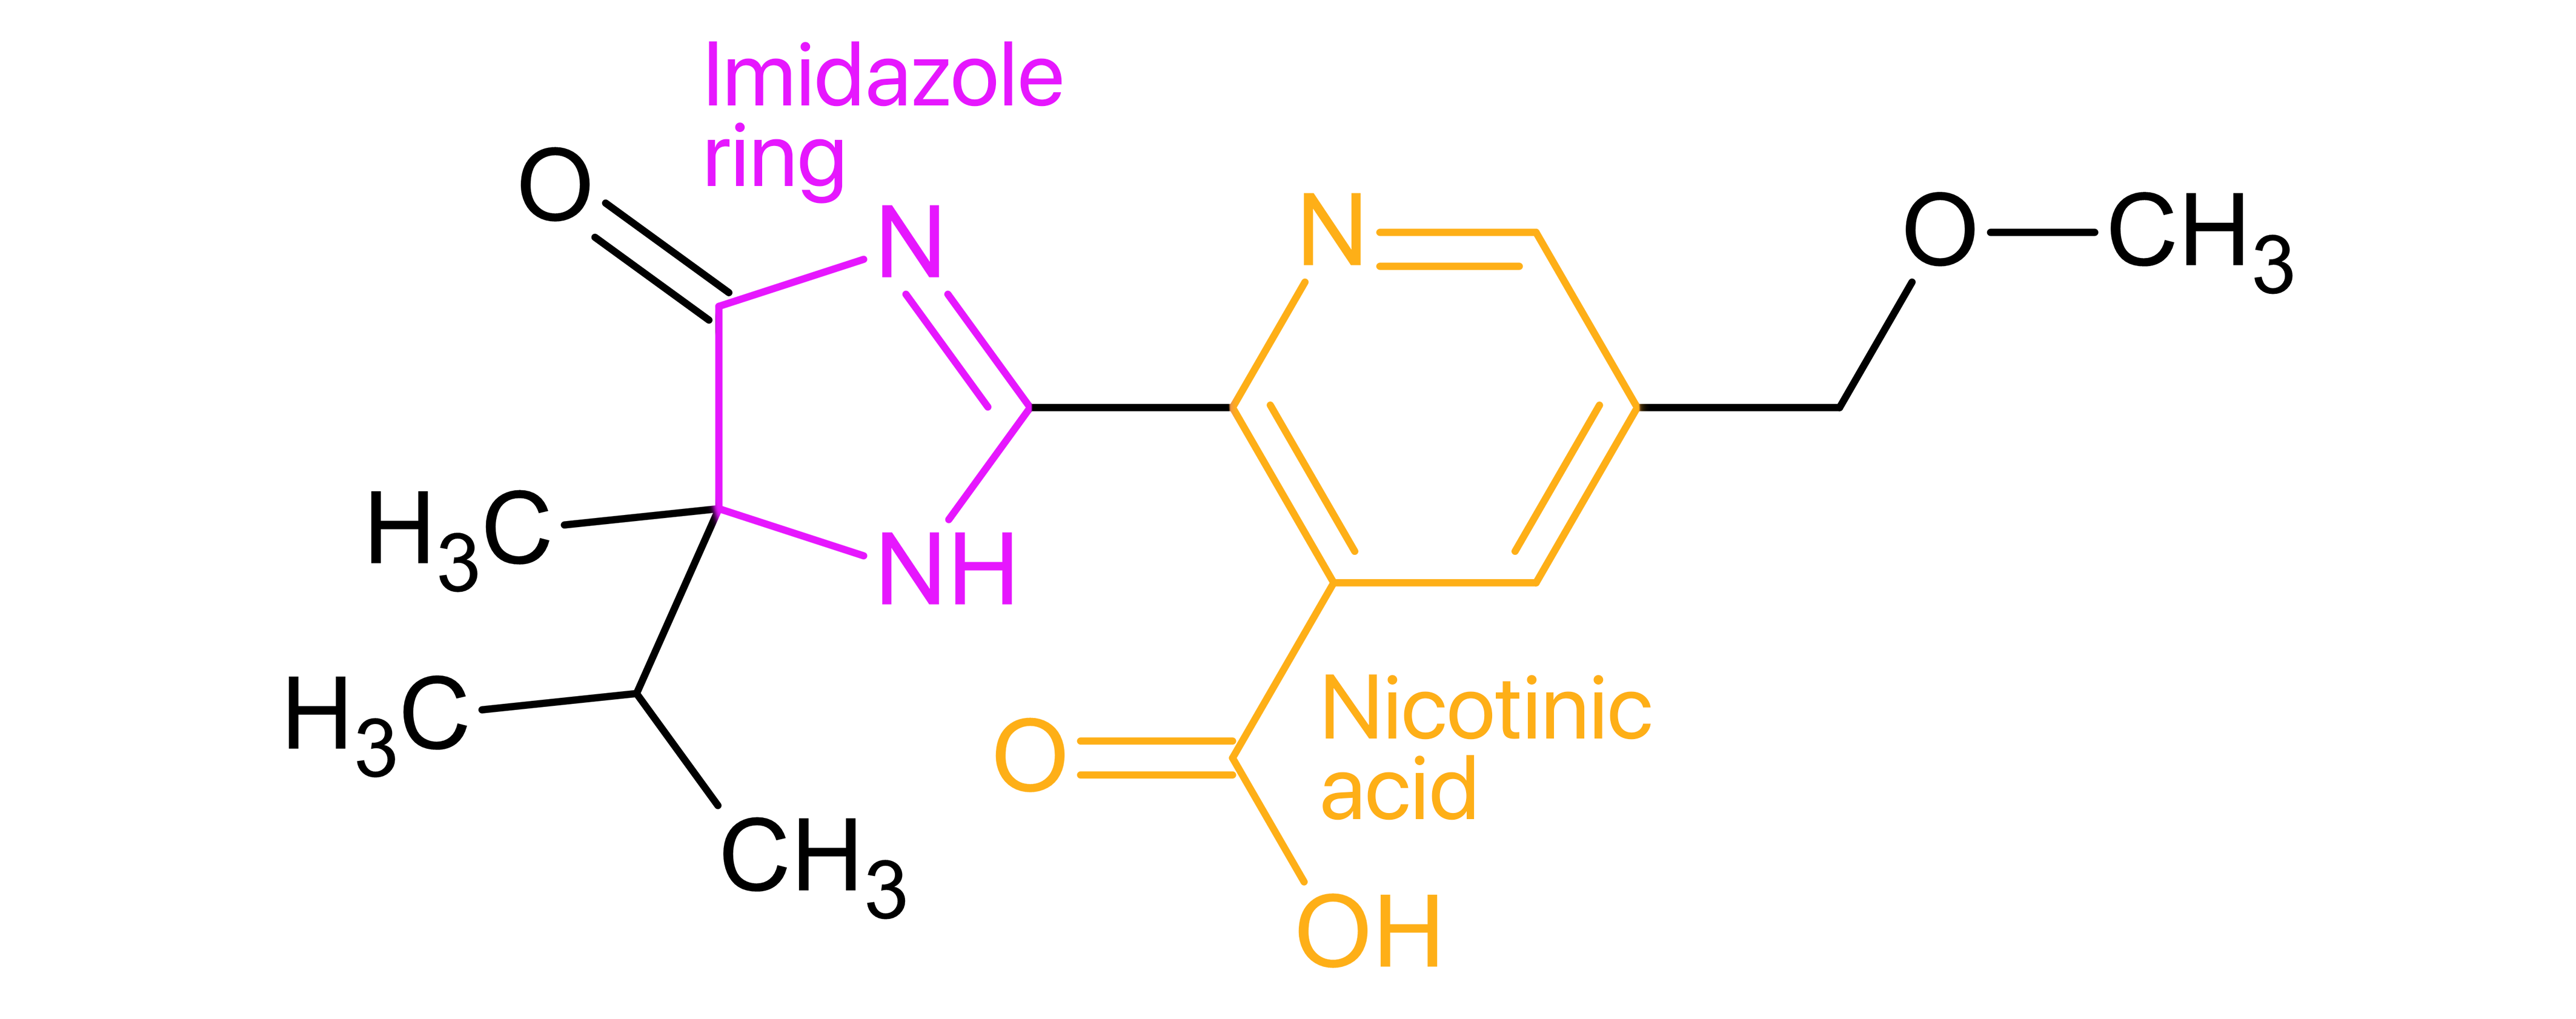
\includegraphics[width=0.8\textwidth]{ESM_Imaz_Structure.png}
\caption{Imazamox structure}
\end{figure}


\newpage


\newpage

\begin{figure}[h!]
\centering
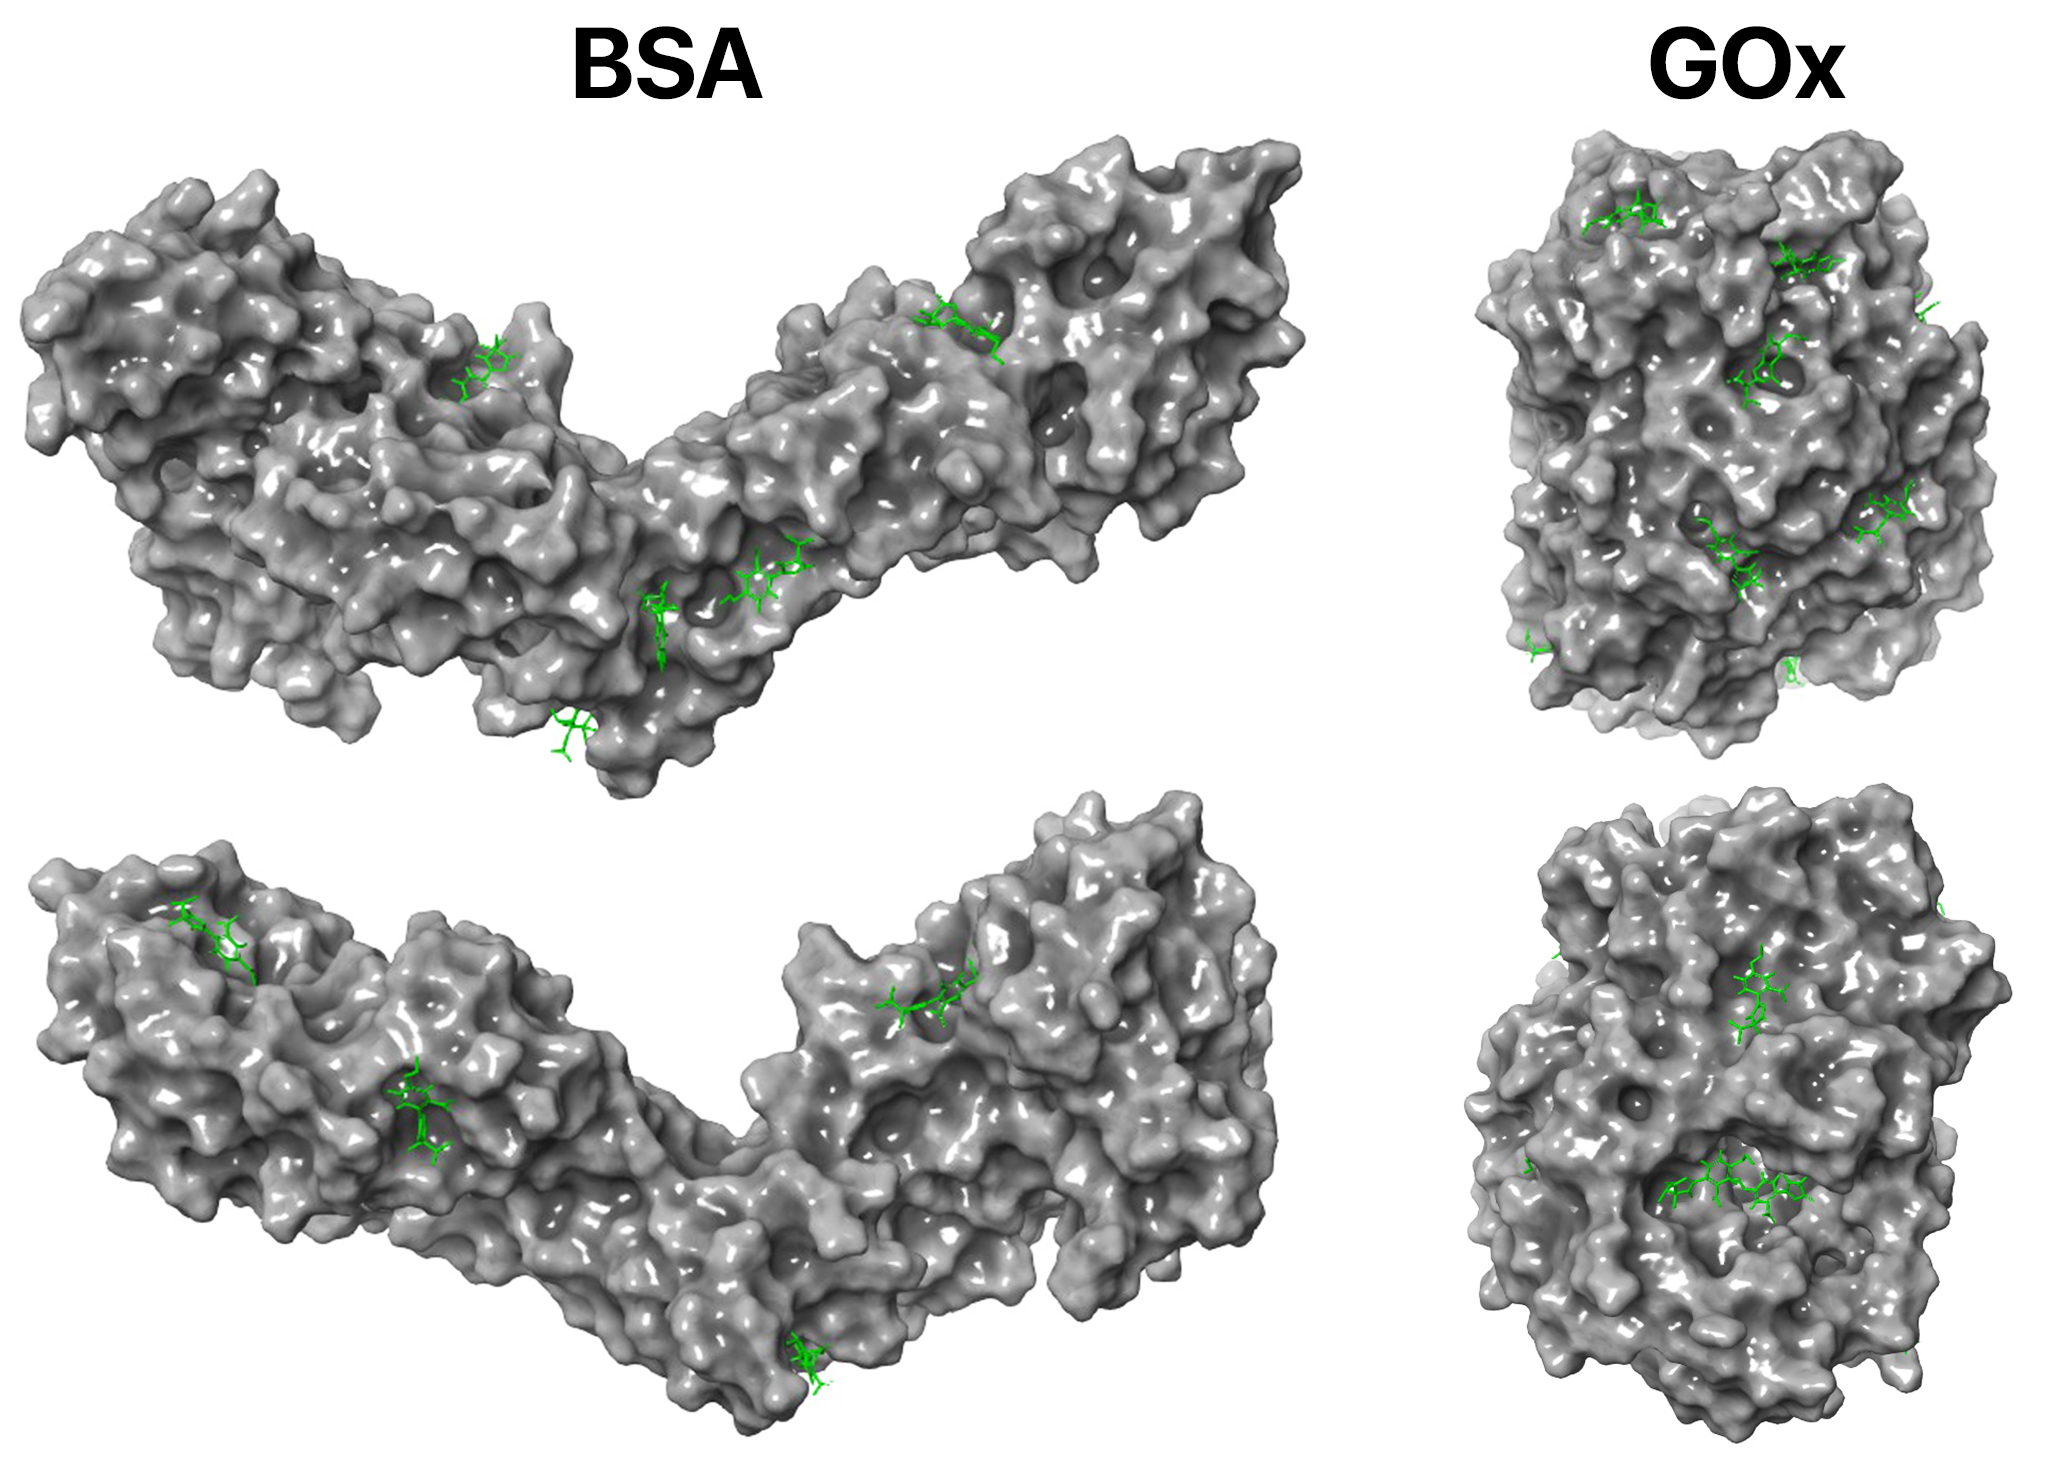
\includegraphics[width=1.0\textwidth]{ESM_Binding_sites.jpg}
\caption{Complex protein--imazamox at pH 3.0}
\end{figure}



\begin{figure}[h!]
\centering
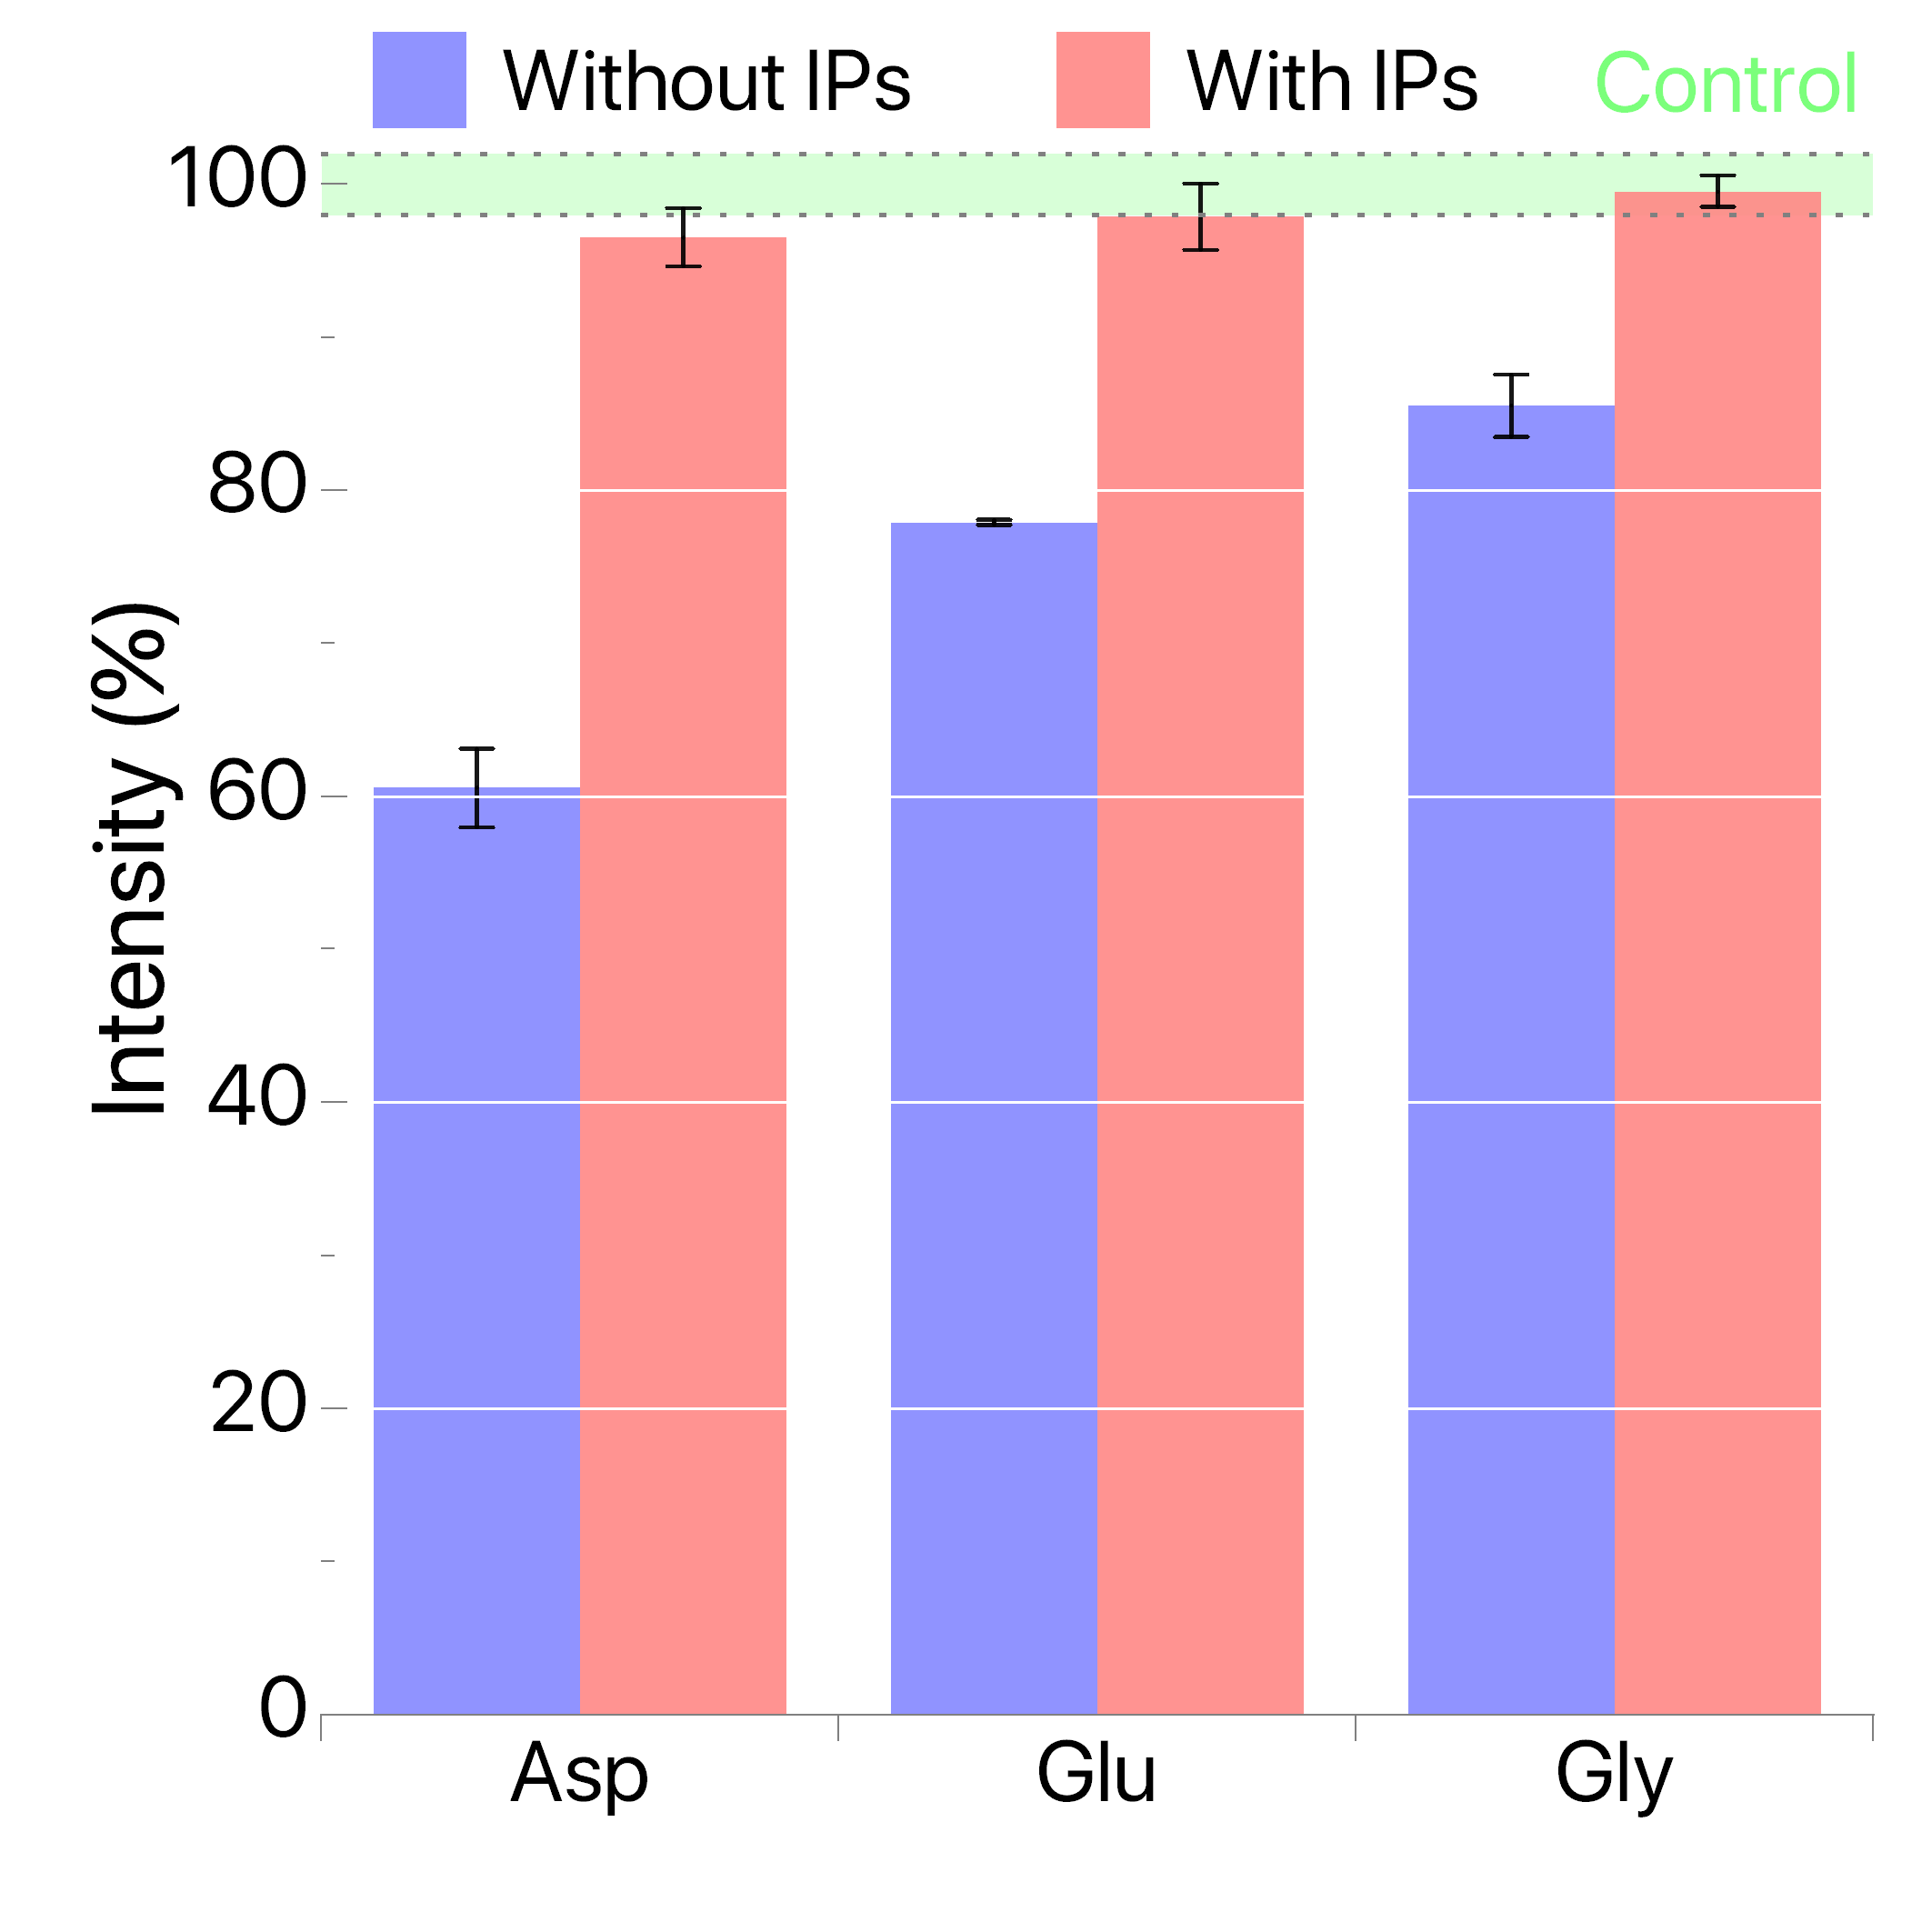
\includegraphics[width=0.5\textwidth]{ESM_AA.png}
\caption{Influence of free amino acids in soil for fluorescence of QDs with and without IPs modification of microplate}
\end{figure}



% \begin{table}[h!]
% \footnotesize
% \centering
% \caption{Analysis of the decay kinetics of CdZnSeS/ZnS QDs with different ligands: OA (in toluene), TGA, MPA and DHLA (in water). The data obtained include values of pure QD colloids and in the presence of MTX (1---100~nM) in water.}
% \begin{tabular}{lrrrrrrrrr}
% \toprule
%          & \textbf{MTX, nM} & \textbf{$\tau_1$, ns} & \textbf{$A_1$, \% }& \textbf{$\tau_2$, ns} & \textbf{$A_2$, \%} & \textbf{$\tau_3$, ns} & \textbf{$A_3$, \%} & \textbf{$\tau_{\text{avg}}$, ns} & \textbf{$\chi^2$}  \\ \midrule

% \textbf{QD\_OA}   & 0       & 3.2    & 30.2   & 11.7   & 64.5   & 71.1   & 5.3    & 29 ± 6         & 1.57 \\ \hline
% \textcolor{blue}{\textbf{QD\_TGA}}  & 0       & 1.4    & 9.4    & 11.9   & 67.7   & 34.5   & 22.9   & 23 ± 1         & 1.13 \\
%          & 1       & 2.1    & 19.2   & 13.4   & 66.7   & 41.4   & 14.2   & 24 ± 2         & 1.14 \\
%  \hline
% \\
% \bottomrule
% \end{tabular}
% \end{table}

% \newpage






\clearpage
\newpage


\clearpage

\newpage





\end{document}
